\section{Conceptual Model}
\label{conceptual_model}

\subsection{Component Model}

We propose and extension to Tropos Model with a component model. By this we aim at creating an appropriate abstraction to allow composable architecture while keeping the traceability between the requirements and implementation at runtime.

Or component model is build around the concept of \textit{strategy}. The strategy at goal model level is a mean of achieving a particular goal. It can have the following realization at runtime:

\begin{itemize}
  \item a strategy can be implemented by a component in the architecture.
  \item can be a delegation to another known agent as a runtime decision.
  \item can be a fault tolerant proxy that combines a implementation or delegation with a fault tolerance technique.
\end{itemize}

From a goal model, each goal will originate at least a capability and strategy. Each OR decomposition of a goal, in the goal model, should correspond to an additional strategy.
An agent in the system has a repository of strategies.

The main concepts are:

\begin{itemize}
  \item \textbf{Agent}: agent is an independent computational unit that manages its own resources (CPU, memory, disk, sensors, etc). After system deployment an agent is turned into an actor of a Tropos model.
  \item \textbf{Capability}: description of a kind of goal that an agent can perform. Its a component interface description in the architecture.
  \item \textbf{Strategy}: a strategy is an alternative way to achieve a goal.
  \item \textbf{Strategy Repository}: an agent has a repository of its known strategies.
\end{itemize}

\begin{figure}
  \centering
  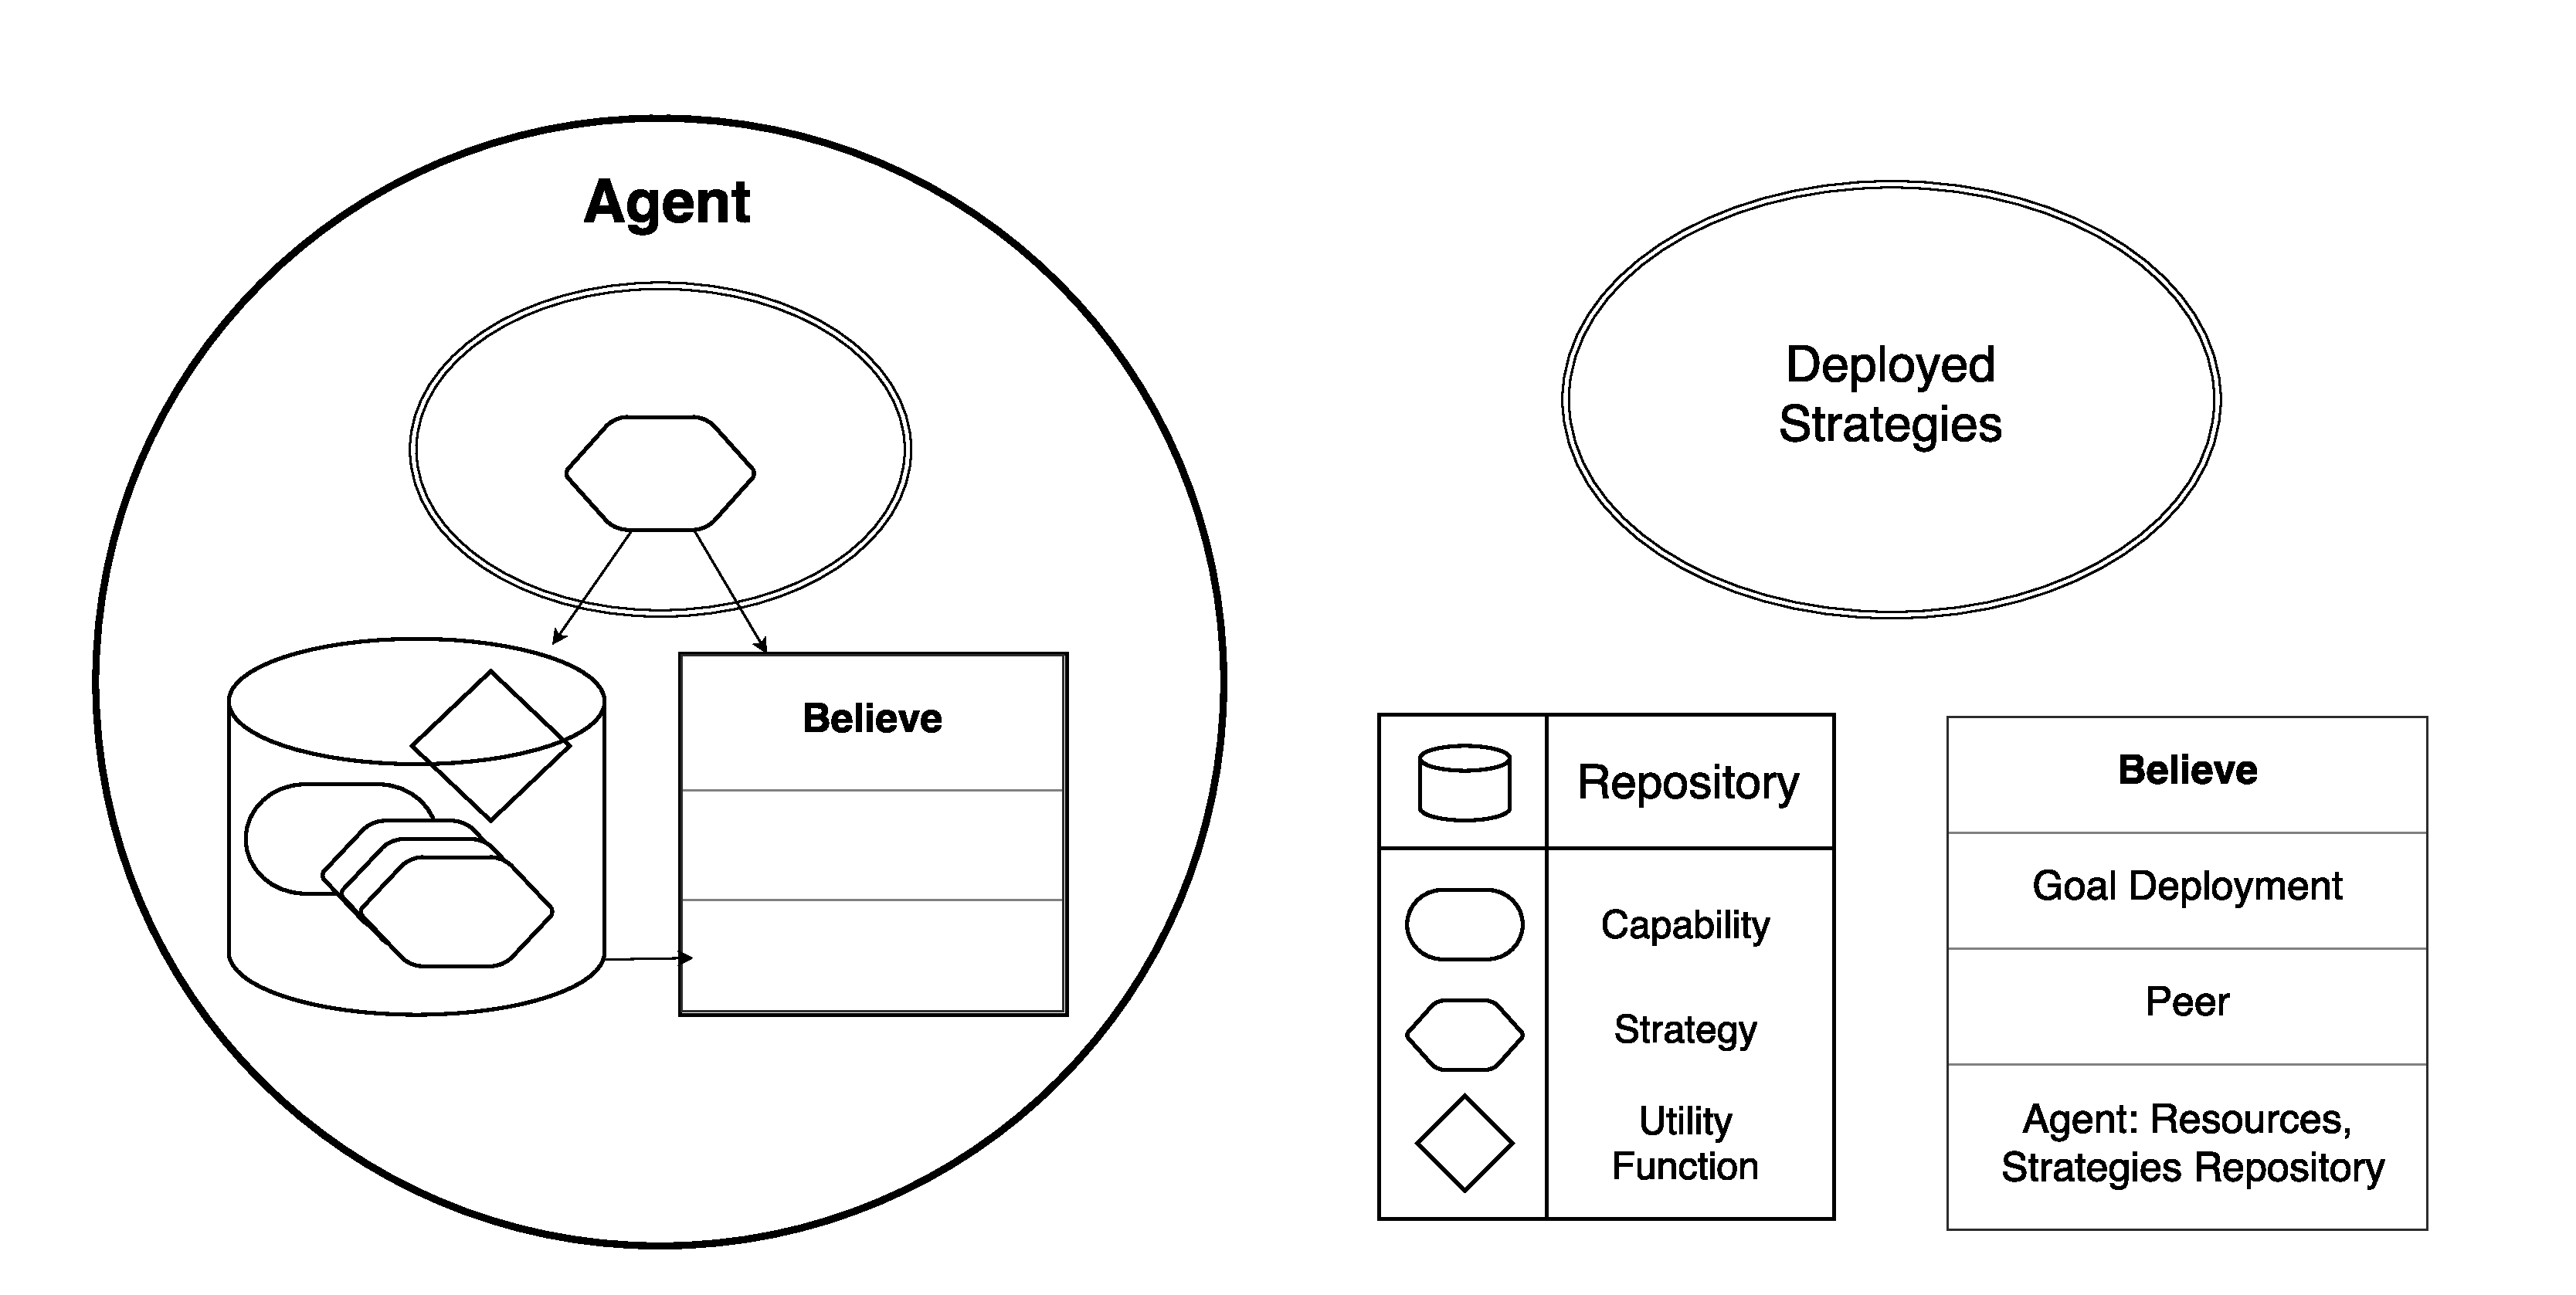
\includegraphics[width=\linewidth]{goalp-agent-repo-rcm-depl}
  \caption{Agent Respresentation}
  \label{fig:goalp-agent}
\end{figure}

A strategy should declare its functional interface by declaring which capability it implements. A strategy also needs to declare its dependencies as plans and capabilities that it depends on. A strategy is active if all its dependencies are currently satisfied. It is inactive otherwise. A capability is satisfied if an agent has at least one active strategy that implement that capability.

\subsection{Architectural Layers}

For the implementation of the conceptual model, we propose an architecture of three layers:

\begin{itemize}
  \item \textbf{Infrastructure}: This layer is responsible for the component model implementation, how capability, strategies, plans and goals instances are described. It also responsible for agent and goals life cycle, strategies management and selection.
  \item \textbf{Adaptation}: This layer is responsible for keep the level of service. It contains strategies to discover peers, team up with peers, gather information to improve strategy selection, etc.
  \item \textbf{Application}: This layer if responsible for functional strategies. The functional strategies are the one that implement user application.
\end{itemize}

\subsection{Runtime Model}

Dalpiaz et al. \cite{dalpiaz_runtime_2013} argue that traditional goal models are not enough for reason about the system at runtime. They propose a distinction between Desgin-time Goal Model (DGM) and Runtime Goal Model (RGM). We extend their proposal of RGM with a component model and runtime strategy selection.

\begin{itemize}

\item \textbf{Goal Instance}: an actual instance of an objective for a given data set.

\item \textbf{Believe}: is the model of an actor about itself and the context. Represents what the agent know.

\item \textbf{Strategy Deployment}: occurs after the strategy selection, is the the binding between the strategy, its capabilities dependencies and its environment dependencies.

\end{itemize}

In the proposed model an actor achieve a goal by \emph{deploying a strategy} and executing it. For instance the deployment of a strategy is a capability itself.

\subsection{Strategy Selection and Deployment}

In order to allow component based adaptation we propose a mechanist of strategy selection at runtime. This mechanism is part of the infrastructure layer. For a hight level of flexibility we propose that the selection mechanism itself should be implemented by components in the architecture.

At a low level an agent has the capability of fulfill goals. Inspired by component based frameworks like Rainbow\cite{garlan_rainbow:_2004} we propose that the strategy should be chosen by means of a utility function. That utility function should be responsible to calculate which available strategy will have a better contribution for softgoals.

After a strategy is selected it is deployed. Strategy deployment corresponds to a component binding in CBSE.

The capability <fulfill goal> and its corresponding strategy should be as follows:

\begin{figure}
  \centering
  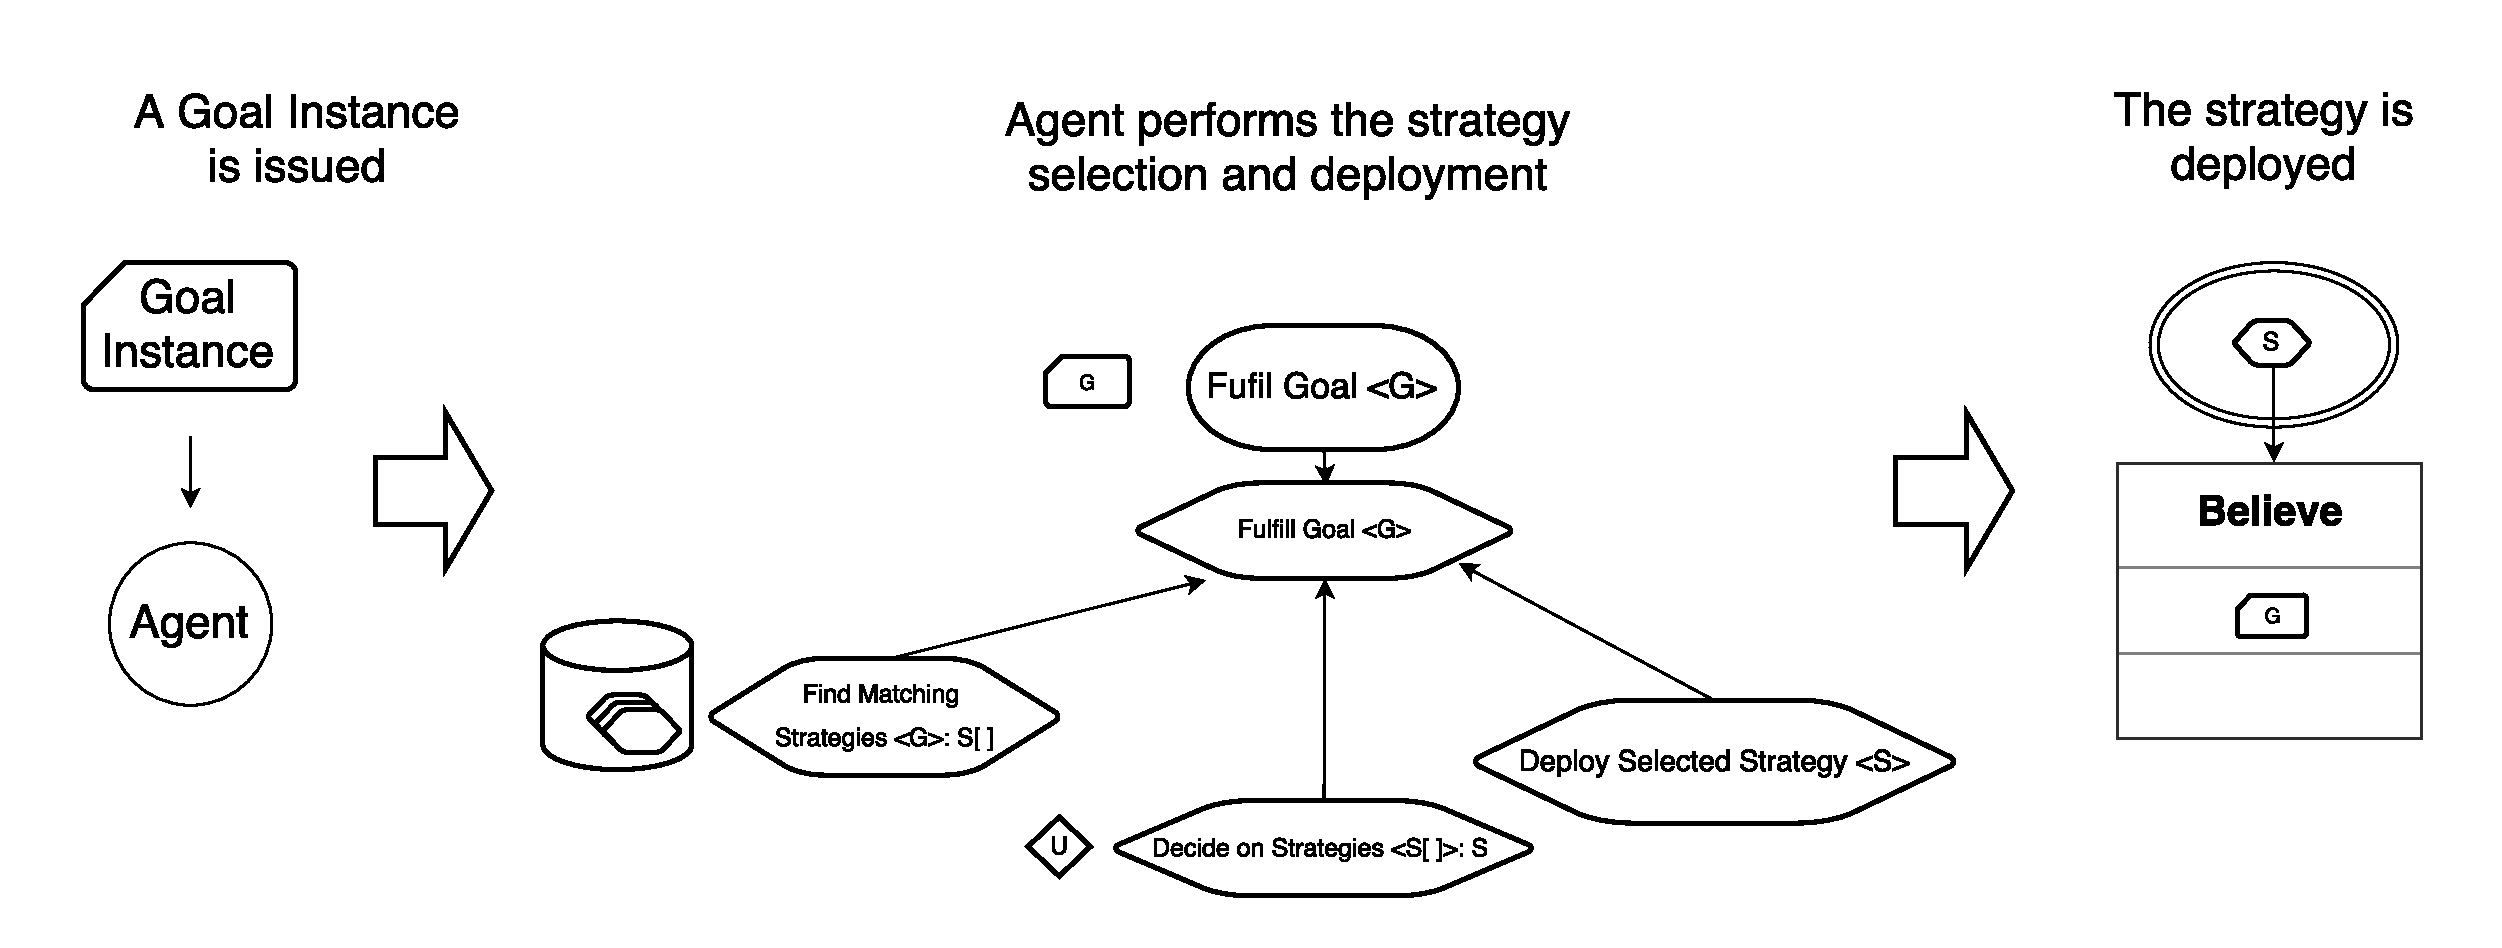
\includegraphics[width=\linewidth]{strategy_deployment}
  \caption{The deployment of a strategy}
  \label{fig:agent_composition}
\end{figure}

\begin{itemize}
\item \textbf{<Fulfill Goals>} the capability to fulfill generic goals.

\item \textbf{<Fulfill Goals>} strategy to fulfill goals by selecting available strategies and evaluating them with an utility function. Consists of 3 sub-goals:
  \begin{itemize}
    \item Find Matching Strategies
    \item Decide on Strategies
    \item Deploy the Selected Strategy
  \end{itemize}
\end{itemize}

And the following three strategies implement the previous 3 capabilities.

\begin{itemize}
  \item \textbf{<Find Local Matching Strategies>} accomplishes <Find Matching Strategies>
  returns the list of matching strategies. A matching strategy is any strategy that implements the goal interface.

  \item \textbf{<Select a Strategy>} accomplishes <Decide on Strategies>
  using a pre-configured utility function that analyses strategies metadata and select a strategy.

  \item \textbf{<Deploy Strategy>} accomplishes <Deploy the Selected Strategy>. Bind the components with the goal instance and dependencies.
\end{itemize}

\subsection{Awareness}

The agent have a model of that repository that it can use for reason about its capabilities, strategies and plans. The agent is also able to manage its own repository.

Self-awareness is provided by a set of self-awareness strategies. Example of self-aware strategies are:

\begin{itemize}
  \item \textbf{<List Local Strategies>}, how the agent can know it actual capabilities.

  \item \textbf{<List Goal Instances>}, how the agent can know it current intentions.

  \item \textbf{<List Deployed Strategies>}, how the agent can know it current running strategies.

\end{itemize}


\subsection{Multi Agent Deployment}

In order to support multi-agent deployments we will extend the conceptual model and create a set of strategies at the adaptation level. First, in the conceptual model, we propose a extension of the Tropos model concept of \textit{role}.

A role, in runtime, will be associated with a set of capabilities. A role is interpreted also as responsibilities of an actor. So if an agent accepts a role it should keep active strategies to accomplish goals related to capabilities associated with its role.
We will call the state when an actor is satisfying all its assigned roles as \textit{satisfying actor}.

The deployment is the process of assign all needed roles to available agents and moving them to a state of satisfying actors.

In order to allow a system to adapt to deployment variability we propose an \textit{actor verification strategy}. With this strategy the actor should check if itself is currently a satisfying actor. If there is a capability that the agent is currently not satisfying it can use \textit{recovery strategies}.

Recovery strategies could be:
\begin{itemize}
  \item lookup for strategy in external strategy repository;
  \item redistribute roles with peers;
  \item lookup for a peer with the missing capability;
  \item restore resource availability;
  %\item degradate the system, making the capability known as not available
\end{itemize}

\subsection{Virtual Strategies}

To extend the model with adaptation capabilities we propose \textif{Virtual Strategies} (VS). VS are means of achieving a goal that is not by binding a component. We propose two kinds of VS:

\begin{itemize}
  \item \textbf{delegating strategies}. VS that allow an agent to achieve a goal by delegating it to a peer agent. When a agent discover that a peer have some capabilities it creates proxy strategies in its own repository that allow it to fulfill goals by delegating to the peer.
  \item \textbf{fault tolerance strategies}. VS that wrap other strategies in a fault tolerance scheme. Examples of possible fault tolerance strategies are \textit{active replication} and \textit{retry}.
\end{itemize}

The creation of virtual strategies will be performed by \textit{Virtual Strategy Producers} (VSP) that are strategies in itself. The creation of a VSP is a \textit{Virtual Strategy Instance} VSI.

A VSI has its own metadata and is evaluated by the utility function in the process of strategy selection.
%TODO For example, if agent has a goal G1, that needs capability C1 to be accomplish and this capability is implemented by strategies S1, S2. An it has also an \textit{active replication VSP} it will chose between deploying S1, S2 or (S1 || S2). In the example, (S1 || S2) been a VSI, the result of active replication of S1 and S2. With this we expect to allow for the development of portable fault tolerance strategies.

% TODO  Strategies and Virtual Strategies can be combined to make flexible solutions at runtime. For example if an actor has a Goal G1, that needs capability C1 to be accomplish and this capability is implemented by strategies S1, S2, S3.

 A VSP can reason about the context in order to adapt the strategy creation. So, for example, in a context that the agent needs to save battery, the active replication strategy may not be produced.
